\documentclass[12pt]{article}
\usepackage[margin=1in]{geometry}
\usepackage{amsmath,amssymb,mathtools}
\usepackage{enumitem}
\usepackage{bm}
\usepackage{hyperref}
\usepackage{fancyhdr}
\usepackage{draftwatermark}
\usepackage{xcolor}
\usepackage{pgfplots}
\usepackage{titlesec}
\pgfplotsset{compat=newest}

%------------- TITLE AND METADATA -------------
\newcommand{\CourseCode}{HE2002 }
\newcommand{\CourseName}{Macroeconomics II}
\newcommand{\DocType}{Tutorial 9}

\title{
\CourseCode \CourseName \\[0.3em]
\large \DocType
}
\author{
  Academic Year 2025/2026, Semester 2 \\[0.25em]
  \textit{Quantitative Research Society @NTU}
}
\date{\today}

%------------- HEADER & FOOTER (for page 2 onward) -------------
\fancypagestyle{main}{
  \fancyhf{}
  \fancyhead[L]{\CourseCode \CourseName \ --\ \DocType}
  \fancyhead[R]{\href{https://qrsntu.org}{QRS@NTU}}
  \fancyfoot[C]{\thepage}
  \renewcommand{\headrulewidth}{0.4pt}
  \renewcommand{\footrulewidth}{0pt}
}

%------------- SIMPLE FOOTER (page 1 only) -------------
\fancypagestyle{plainfirst}{
  \fancyhf{}
  \renewcommand{\headrulewidth}{0pt}
  \renewcommand{\footrulewidth}{0pt}
  \fancyfoot[C]{\scriptsize\textcolor{gray}{\textit{For academic reference only. This document is provided for educational purposes and does not constitute an official question paper, answer key, or any formally authorised academic material. Its content is not guaranteed to be complete or accurate.}}}
}

%------------- WATERMARK -------------
\SetWatermarkText{Unofficial — QRS@NTU — qrsntu.org}
\SetWatermarkScale{1}
\SetWatermarkLightness{0.99}

%------------- SHORTCUTS -------------
\newcommand{\R}{\mathbb{R}}
\newcommand{\Rp}{\mathbb{R}_+}
\newcommand{\E}{\mathbb{E}}
\newcommand{\Var}{\mathrm{Var}}
\newcommand{\dotp}{\cdot}

%------------- STYLE -------------
\setlist[enumerate]{itemsep=0.32em, topsep=0.32em}
\setlist[itemize]{itemsep=0.22em, topsep=0.22em}

\titleformat{\subsubsection}[block]
{\normalfont\large\bfseries}
{}
{0pt}
{}

\titleformat{\paragraph}[block]
{\normalfont\normalsize\bfseries}
{}
{0pt}
{}

\titlespacing*{\paragraph}
{0pt}
{1.2ex}
{0.6ex}

\setcounter{secnumdepth}{0}
\setcounter{tocdepth}{4}

\begin{document}

\maketitle
\thispagestyle{plainfirst}
\pagestyle{main}
\bigskip

%====================================================
% OVERVIEW
%====================================================
\begin{center}
  \rule{0.8\textwidth}{0.4pt}\\[4pt]
  \textbf{Overview}\\[2pt]
  \rule{0.8\textwidth}{0.4pt}
\end{center}

\noindent
This tutorial covers:
\begin{itemize}[leftmargin=*]
  \item linear production technologies, returns to scale, and the output-per-worker representation;
  \item growth-accounting logic for economies in which output depends on capital accumulation alone;
  \item the implications of diminishing returns for sustaining long-run growth;
  \item the Cobb--Douglas production function, including constant returns to scale and diminishing partial returns;
  \item per-worker transformations and the geometry of production functions in macroeconomics.
\end{itemize}

\bigskip

\newpage
\tableofcontents

\newpage
%====================================================
% QUESTION 1
%====================================================
\section{Question 1: Linear Production Function and Output per Worker}

\noindent
Chapter 10, Q3

\subsection{Problem}
Consider the production function:
\[
Y = K + 2N
\]
\begin{enumerate}[label=(\alph*)]
    \item Compute output when \(K = 10\) and \(N = 20\).
    \item If both capital and labor triple, what happens to output?
    \item How would you qualify the returns to scale for this production function?
    \item Write this production function as a relation between output per worker and capital per worker.
    \item Let \(K/N = 2\). What is \(Y /N\)? Now double \(K/N = 4\). Does \(Y /N\) double as a result?
    \item In the per worker form of the production function, what does it tell us about the marginal return to capital per woker?
    \item Plot the relation between output per worker and capital per worker. How does the shape of this relationship compare with the figure on Slide 21, Output and Capital per Worker?
\end{enumerate}

\subsection{Solution}

\subsubsection{Method 1: Direct substitution and scaling analysis}
\begin{enumerate}[label=(\alph*)]
    \item
    Substitute \(K=10\) and \(N=20\) into
    \[
    Y=K+2N.
    \]
    Then
    \[
    Y=10+2(20)=10+40=50.
    \]
    Therefore,
    \[
    \boxed{Y=50.}
    \]

    \item
    If both capital and labor triple, then \((K,N)\mapsto(3K,3N)\). Output becomes
    \[
    Y'=3K+2(3N)=3K+6N=3(K+2N)=3Y.
    \]
    Hence output also triples.
    \[
    \boxed{\text{If both inputs triple, output triples.}}
    \]

    \item
    A production function has constant returns to scale if multiplying all inputs by the same positive factor \(\lambda\) multiplies output by exactly \(\lambda\). Here
    \[
    F(K,N)=K+2N.
    \]
    For any \(\lambda>0\),
    \[
    F(\lambda K,\lambda N)=\lambda K+2\lambda N=\lambda(K+2N)=\lambda F(K,N).
    \]
    Hence the production function is characterized by constant returns to scale.
    \[
    \boxed{\text{The production function has constant returns to scale.}}
    \]

    \item
    Divide both sides of
    \[
    Y=K+2N
    \]
    by \(N\) (assuming \(N>0\)):
    \[
    \frac{Y}{N}=\frac{K}{N}+2.
    \]
    If we define output per worker by
    \[
    y:=\frac{Y}{N}
    \]
    and capital per worker by
    \[
    k:=\frac{K}{N},
    \]
    then the per worker production function is
    \[
    y=k+2.
    \]
    Therefore,
    \[
    \boxed{\frac{Y}{N}=\frac{K}{N}+2 \quad\text{or}\quad y=k+2.}
    \]

    \item
    First let
    \[
    \frac{K}{N}=2.
    \]
    Then from the per worker form,
    \[
    \frac{Y}{N}=\frac{K}{N}+2=2+2=4.
    \]
    Now double \(\frac{K}{N}\) to \(4\). Then
    \[
    \frac{Y}{N}=4+2=6.
    \]
    So output per worker rises from \(4\) to \(6\), not from \(4\) to \(8\). Thus it does not double.
    \[
    \boxed{\text{If }K/N=2,\ Y/N=4;\ \text{if }K/N=4,\ Y/N=6;\ \text{so }Y/N\text{ does not double.}}
    \]

    \item
    In per worker form,
    \[
    y=k+2.
    \]
    The marginal return to capital per worker is the slope of this function:
    \[
    \frac{dy}{dk}=1.
    \]
    So the marginal return to capital per worker is constant. It does not decline as \(k\) rises.
    \[
    \boxed{\frac{dy}{dk}=1,\ \text{so the marginal return to capital per worker is constant, not diminishing.}}
    \]

    \item
    The relation between output per worker and capital per worker is the straight line
    \[
    y=k+2,
    \]
    which has vertical intercept \(2\) and slope \(1\).

    A correct plot is therefore:

    \begin{center}
    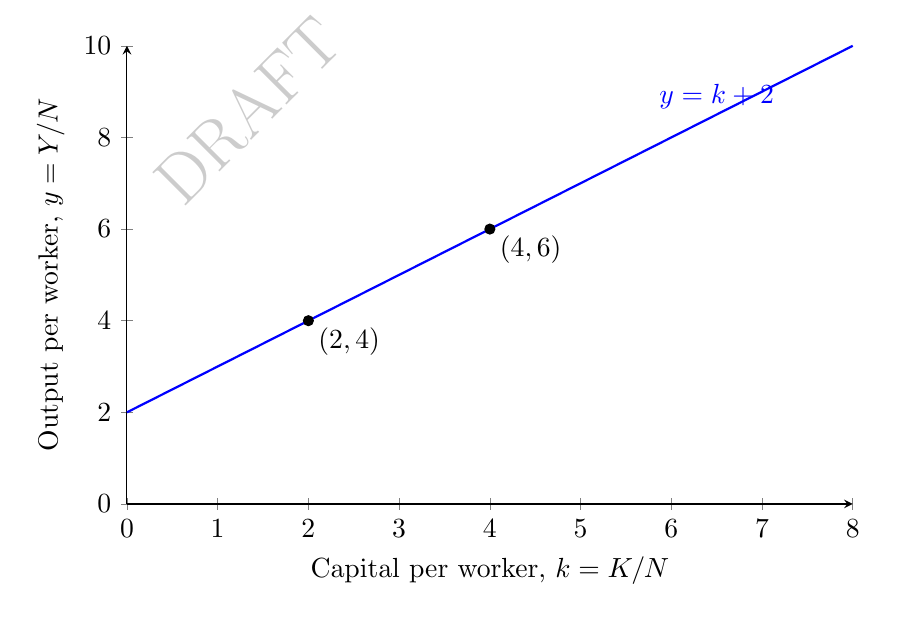
\begin{tikzpicture}
    \begin{axis}[
        width=10.8cm,
        height=7.4cm,
        xmin=0,xmax=8,
        ymin=0,ymax=10,
        axis lines=left,
        xlabel={Capital per worker, \(k=K/N\)},
        ylabel={Output per worker, \(y=Y/N\)},
        xtick={0,1,2,3,4,5,6,7,8},
        ytick={0,2,4,6,8,10},
        clip=false
    ]
    \addplot[domain=0:8,samples=2,thick,blue] {x+2};
    \node[blue] at (axis cs:6.5,8.9) {\(y=k+2\)};
    \addplot[only marks,mark=*,mark size=1.8pt] coordinates {(2,4) (4,6)};
    \node at (axis cs:2.45,3.55) {\((2,4)\)};
    \node at (axis cs:4.45,5.55) {\((4,6)\)};
    \end{axis}
    \end{tikzpicture}
    \end{center}

    Compared with the standard figure on Slide 21, this relationship is not concave. Instead of flattening out as \(k\) rises, it is linear with constant slope. So unlike the standard neoclassical case, this technology does not display diminishing returns to capital per worker.
    \[
    \boxed{\text{The graph is a straight line, whereas the standard slide figure is concave and flattening.}}
    \]
\end{enumerate}

\subsubsection{Method 2: Per-worker and homogeneity method}
\begin{enumerate}[label=(\alph*)]
    \item
    Since output is
    \[
    Y=K+2N,
    \]
    each unit of capital contributes \(1\) unit of output and each unit of labor contributes \(2\) units of output. Hence with \(K=10\) and \(N=20\),
    \[
    Y=10+40=50.
    \]
    Therefore,
    \[
    \boxed{Y=50.}
    \]

    \item
    If both inputs triple, output can be found directly from the per-worker logic. When both \(K\) and \(N\) triple, capital per worker stays unchanged:
    \[
    \frac{3K}{3N}=\frac{K}{N}.
    \]
    So output per worker stays the same. But because the number of workers triples, total output triples as well:
    \[
    Y' = 3Y.
    \]
    Hence
    \[
    \boxed{\text{Output triples.}}
    \]

    \item
    The previous argument is precisely the content of constant returns to scale: if all inputs scale by the same factor, total output scales by the same factor. Therefore,
    \[
    \boxed{\text{The technology exhibits constant returns to scale.}}
    \]

    \item
    Divide by \(N\):
    \[
    \frac{Y}{N}=\frac{K}{N}+2.
    \]
    Writing \(y=Y/N\) and \(k=K/N\),
    \[
    \boxed{y=k+2.}
    \]

    \item
    The per-worker representation answers this immediately. If \(k=2\), then
    \[
    y=2+2=4.
    \]
    If \(k=4\), then
    \[
    y=4+2=6.
    \]
    Hence \(y\) rises by \(2\), not by a factor of \(2\):
    \[
    \boxed{y(2)=4,\quad y(4)=6,\quad \text{so output per worker does not double.}}
    \]

    \item
    In the graph of \(y\) against \(k\), the marginal return to capital per worker is the slope. Since
    \[
    y=k+2,
    \]
    the slope is constant and equal to \(1\) everywhere. Therefore there is no diminishing marginal return to capital per worker:
    \[
    \boxed{\text{The marginal return to capital per worker is constant and equal to }1.}
    \]

    \item
    The graph is the line \(y=k+2\). Its key geometric features are:
    \begin{itemize}[leftmargin=*]
        \item intercept \(2\) on the \(y\)-axis;
        \item constant slope \(1\);
        \item no curvature;
        \item no flattening as \(k\) increases.
    \end{itemize}
    Hence, relative to the standard neoclassical figure on Slide 21, the present graph is much steeper at high values of \(k\) and does not bend downward.
    \[
    \boxed{\text{This graph is linear, unlike the usual concave output-per-worker curve.}}
    \]
\end{enumerate}

\newpage
%====================================================
% QUESTION 2
%====================================================
\section{Question 2: The Growth Rates of Capital and Output}

\noindent
Chapter 10, Q4 The growth rates of capital and output

\subsection{Problem}
Consider the production function given by
\[
Y=\sqrt{K}\sqrt{N}.
\]
Assume that \(N\) is constant and equal to 1. Note that if \(z=x^a\), then \(g_z\approx ag_x\), where \(g_z\) and \(g_x\) are the growth rates of \(z\) and \(x\) (See Appendix 2 at the end of the book).

\begin{enumerate}[label=(\alph*)]
    \item Given the growth approximation here, derive the relation between the growth rate of output and the growth rate of capital.
    \item Suppose we want to achieve output growth equal to 2\% per year. What is the required rate of growth of capital?
    \item In part b, what happens to the ratio of capital to output over time?
    \item Is it possible to sustain output growth of 2\% forever in this economy? Why or why not?
\end{enumerate}

\subsection{Solution}

\subsubsection{Method 1: Growth-accounting approximation}
Because \(N=1\) is constant, we have
\[
Y=\sqrt{K}\sqrt{1}=\sqrt{K}=K^{1/2}.
\]

\begin{enumerate}[label=(\alph*)]
    \item
    Using the approximation
    \[
    g_z\approx ag_x \quad \text{when } z=x^a,
    \]
    and applying it to
    \[
    Y=K^{1/2},
    \]
    we obtain
    \[
    g_Y\approx \frac{1}{2}g_K.
    \]
    Therefore,
    \[
    \boxed{g_Y\approx \frac{1}{2}g_K.}
    \]

    \item
    If the target is
    \[
    g_Y=2\%,
    \]
    then
    \[
    2\%\approx \frac{1}{2}g_K.
    \]
    Multiplying both sides by \(2\),
    \[
    g_K\approx 4\%.
    \]
    Hence the required capital growth rate is
    \[
    \boxed{g_K\approx 4\%\text{ per year.}}
    \]

    \item
    The capital-output ratio is
    \[
    \frac{K}{Y}.
    \]
    Growth-rate arithmetic gives
    \[
    g_{K/Y}=g_K-g_Y.
    \]
    Using part (b),
    \[
    g_{K/Y}\approx 4\%-2\%=2\%.
    \]
    So the capital-output ratio rises over time at approximately 2\% per year.
    \[
    \boxed{\frac{K}{Y}\text{ increases over time, at approximately }2\%\text{ per year.}}
    \]

    \item
    In this economy, output growth comes only from capital accumulation, and the production function
    \[
    Y=K^{1/2}
    \]
    exhibits diminishing returns to capital. To keep output growing at 2\% forever, capital must keep growing at 4\% forever. But then the capital-output ratio keeps rising forever, as part (c) showed.

    This means ever more capital is needed for each extra unit of output. Equivalently, because marginal product falls as \(K\) rises, sustaining the same output growth rate requires an increasingly large amount of investment relative to output. In a standard macroeconomic setting, that is not sustainable forever without technological progress.

    Therefore,
    \begin{center}
    \fbox{\parbox{0.9\linewidth}{\centering
    No. A $2\%$ output growth rate cannot be sustained forever because diminishing returns to capital require an ever-rising $K/Y$ ratio.
    }}
    \end{center}
\end{enumerate}

\subsubsection{Method 2: Exact transformation and ratio analysis}
Since \(N=1\), the production function simplifies exactly to
\[
Y=\sqrt{K}.
\]
Squaring both sides gives
\[
Y^2=K.
\]

\begin{enumerate}[label=(\alph*)]
    \item
    Differentiate logarithmically. From
    \[
    \ln Y=\frac{1}{2}\ln K,
    \]
    we obtain
    \[
    g_Y=\frac{1}{2}g_K
    \]
    exactly in continuous-time growth notation and approximately in discrete-time growth rates. Hence
    \[
    \boxed{g_Y\approx \frac{1}{2}g_K.}
    \]

    \item
    To achieve
    \[
    g_Y=2\%,
    \]
    the relation above implies
    \[
    \frac{1}{2}g_K=2\%.
    \]
    Therefore
    \[
    \boxed{g_K=4\%.}
    \]

    \item
    Using \(Y=\sqrt{K}\), the capital-output ratio is
    \[
    \frac{K}{Y}=\frac{K}{\sqrt{K}}=\sqrt{K}=Y.
    \]
    Thus the capital-output ratio grows at exactly the same rate as output:
    \[
    g_{K/Y}=g_Y=2\%.
    \]
    Hence
    \[
    \boxed{\frac{K}{Y}\text{ rises over time, growing at }2\%\text{ per year.}}
    \]

    \item
    A sharper way to see the sustainability issue is through required investment. Ignoring depreciation for the logic of the argument, sustaining
    \[
    g_K=4\%
    \]
    requires net investment of about
    \[
    I \approx 0.04K.
    \]
    Relative to output,
    \[
    \frac{I}{Y}\approx 0.04\frac{K}{Y}.
    \]
    But part (c) shows that \(K/Y\) rises forever. Therefore \(I/Y\) must also rise forever. In particular, the share of output that must be devoted to investment becomes arbitrarily large, which is not feasible in a standard economy.

    So,
    \begin{center}
    \fbox{\parbox{0.9\linewidth}{\centering
    No. Sustaining $2\%$ output growth forever would require an ever-increasing investment burden because $K/Y$ keeps rising.
    }}
    \end{center}
\end{enumerate}

\newpage
%====================================================
% QUESTION 3
%====================================================
\section{Question 3: The Cobb--Douglas Production Function}

\noindent
Chapter 11, Q7. The Cobb-Douglas production function. (a)-(d)

\subsection{Problem}
Suppose that the economy’s production function is given by
\[
Y=K^\alpha N^{1-\alpha}
\]
and assume that \(\alpha=1/3\)

\begin{enumerate}[label=(\alph*)]
    \item Is this production function characterized by constant returns to scale? Explain.
    \item Are there decreasing returns to capital?
    \item Are there decreasing returns to labor?
    \item Transform the production function into a relation between output per worker and capital per worker.
\end{enumerate}

\subsection{Solution}

\subsubsection{Method 1: Direct exponent algebra}
Since \(\alpha=1/3\), the production function is
\[
Y=K^{1/3}N^{2/3}.
\]

\begin{enumerate}[label=(\alph*)]
    \item
    To test for returns to scale, multiply both inputs by \(\lambda>0\):
    \[
    F(\lambda K,\lambda N)
    =(\lambda K)^{1/3}(\lambda N)^{2/3}
    =\lambda^{1/3}\lambda^{2/3}K^{1/3}N^{2/3}
    =\lambda K^{1/3}N^{2/3}.
    \]
    Hence
    \[
    F(\lambda K,\lambda N)=\lambda F(K,N).
    \]
    Therefore the production function has constant returns to scale.
    \[
    \boxed{\text{Yes. The production function has constant returns to scale.}}
    \]

    \item
    To examine returns to capital, hold \(N\) fixed. Then
    \[
    Y=N^{2/3}K^{1/3}.
    \]
    If capital doubles while labor is fixed, output becomes
    \[
    Y' = N^{2/3}(2K)^{1/3}=2^{1/3}N^{2/3}K^{1/3}=2^{1/3}Y.
    \]
    Since
    \[
    2^{1/3}<2,
    \]
    output rises by less than proportionately with capital. Thus there are decreasing returns to capital.

    Equivalently,
    \[
    MP_K=\frac{\partial Y}{\partial K}
    =\frac{1}{3}K^{-2/3}N^{2/3},
    \]
    which falls as \(K\) rises.

    Therefore,
    \[
    \boxed{\text{Yes. There are decreasing returns to capital.}}
    \]

    \item
    Hold \(K\) fixed. Then
    \[
    Y=K^{1/3}N^{2/3}.
    \]
    If labor doubles while capital is fixed, output becomes
    \[
    Y'=K^{1/3}(2N)^{2/3}=2^{2/3}K^{1/3}N^{2/3}=2^{2/3}Y.
    \]
    Since
    \[
    2^{2/3}<2,
    \]
    output rises by less than proportionately with labor. Thus there are decreasing returns to labor.

    Equivalently,
    \[
    MP_N=\frac{\partial Y}{\partial N}
    =\frac{2}{3}K^{1/3}N^{-1/3},
    \]
    which falls as \(N\) rises.

    Therefore,
    \[
    \boxed{\text{Yes. There are decreasing returns to labor.}}
    \]

    \item
    Divide the production function by \(N\):
    \[
    \frac{Y}{N}
    =
    \frac{K^{1/3}N^{2/3}}{N}
    =
    K^{1/3}N^{-1/3}.
    \]
    Rearranging,
    \[
    \frac{Y}{N}=\left(\frac{K}{N}\right)^{1/3}.
    \]
    If we write
    \[
    y:=\frac{Y}{N},
    \qquad
    k:=\frac{K}{N},
    \]
    then the per worker production function is
    \[
    y=k^{1/3}.
    \]
    Hence,
    \[
    \boxed{\frac{Y}{N}=\left(\frac{K}{N}\right)^{1/3}\quad\text{or}\quad y=k^{1/3}.}
    \]
\end{enumerate}

\subsubsection{Method 2: Homogeneity, marginal products, and log form}
Again, with \(\alpha=1/3\), we have
\[
Y=K^{1/3}N^{2/3}.
\]

\begin{enumerate}[label=(\alph*)]
    \item
    The sum of exponents is
    \[
    \frac{1}{3}+\frac{2}{3}=1.
    \]
    For a Cobb--Douglas production function, exponents summing to \(1\) imply homogeneity of degree \(1\), which is exactly constant returns to scale.

    To verify it explicitly,
    \[
    \ln Y=\frac{1}{3}\ln K+\frac{2}{3}\ln N.
    \]
    Replacing \(K\) and \(N\) by \(\lambda K\) and \(\lambda N\),
    \[
    \ln F(\lambda K,\lambda N)
    =
    \frac{1}{3}\ln(\lambda K)+\frac{2}{3}\ln(\lambda N)
    =
    \left(\frac{1}{3}+\frac{2}{3}\right)\ln\lambda + \ln F(K,N),
    \]
    so
    \[
    \ln F(\lambda K,\lambda N)=\ln \lambda + \ln F(K,N).
    \]
    Exponentiating gives
    \[
    F(\lambda K,\lambda N)=\lambda F(K,N).
    \]
    Therefore,
    \[
    \boxed{\text{Yes. The technology has constant returns to scale.}}
    \]

    \item
    Decreasing returns to capital means that, with labor fixed, the marginal product of capital declines as \(K\) increases. Here
    \[
    MP_K=\frac{\partial Y}{\partial K}
    =\frac{1}{3}K^{-2/3}N^{2/3}.
    \]
    Because the exponent on \(K\) is negative in \(MP_K\), the marginal product falls as \(K\) rises. So there are decreasing returns to capital:
    \[
    \boxed{\text{Yes. There are decreasing returns to capital.}}
    \]

    \item
    Likewise,
    \[
    MP_N=\frac{\partial Y}{\partial N}
    =\frac{2}{3}K^{1/3}N^{-1/3}.
    \]
    Since the exponent on \(N\) is negative in \(MP_N\), the marginal product of labor falls as labor rises. Thus there are decreasing returns to labor:
    \[
    \boxed{\text{Yes. There are decreasing returns to labor.}}
    \]

    \item
    Divide by \(N\):
    \[
    y=\frac{Y}{N}=K^{1/3}N^{-1/3}.
    \]
    Using exponent rules,
    \[
    K^{1/3}N^{-1/3}=\left(\frac{K}{N}\right)^{1/3}.
    \]
    Therefore the output-per-worker relation is
    \[
    \boxed{y=k^{1/3}.}
    \]
    This is the standard concave per-worker production function: it rises with \(k\), but at a decreasing rate.
\end{enumerate}

\end{document}
